\chapter{Tested Material}

With the requirements discussed in the previous chapter in mind the material that would be tested were chosen.

%%%%%%%%%%%%%%%
%Concrete
\section*{Concrete}
%TO DO more concrete information
The concrete used in the tested sample %was almost exclusively 
fibre reinforced with approximately 40 \(\frac{\text{kg}}{\text{m}^3}\) of steel fibres. Its hardness class was C50, it has a UCS of 50 MPa.

%Its cement was produced by X

%The aggregates are sourced from Y.

%%%%%
%Mesh
\section*{Welded Mesh}
The welded mesh has a wire diameter of \o 5,5 mm and c/c 75 mm. It is used in 2,2 on 2,3 m sheets. 

\section*{Textile Mesh}
The textile mesh that was be tested is manufactured by Huesker and is called minegrid. 

%%%%%%%%
\section*{Chain-Link Mesh}

Special attention has to be given to the plates used with chain-link mesh. As the wire are quite thin, they are prone to breaking when used in conjunction with a flat plate. \textcite{chainlink11} suggests using special spiked plates.
%As the number of available samples was quite small, chain-link mesh will not be tested.

%%%%%%%%%%%%%%
\section*{Fjällband}
\label{sec:fjäll}

\begin{figure}
    \centering
    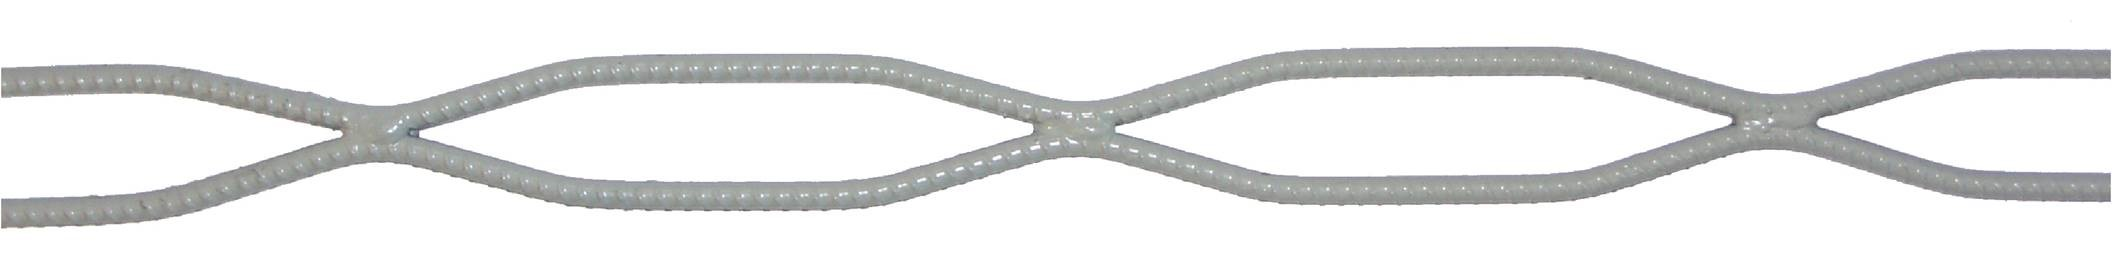
\includegraphics[width=0.95\linewidth]{pics/Fjallband.jpg}
    \caption{A sketch of Fjällband}
    \label{fig:fjäll}
\end{figure}

Fjällband is a type of strap. It is manufactured in-house and has to be installed manually which is time and cost intensive. Its effects on the rock support have not been studied so far. It consists of two wavy metal rods that are welded together at their peaks, see \autoref{fig:fjäll}.  %implementing a different type of lacing which could be installed in at least a mechanised if not automized way would be more efficient. 

%%%%%%%%%%%%%%%
%Lacing
\section*{Lacing}
Only wire rope will be tested, though it might be interesting to consider rope made from nylon or polyester in the future. Of course the diameter and the deformability would increase but it would be lighter, easier to handle and would not suffer corrosion. Fire might pose a large risk to synthetic rope. If lacing were to be deployed across large areas in the mine it might be worth considering "exotic" materials, such as nylon or polyester. Umeå university and LKAB started  a joint project to investigate using synthetic materials for hoist cables instead of steel. The results of this project were not available when the test matrix of this thesis was planned.
The results from these investigations could be used for future tests. %It has not yet been tested.
For the current experiments galvanized steel wire (6 x 24 + 7FC) was used. It had a breaking load of 43.9 kN. The technical data sheet can be found in the appendix.

%%%%%%%
\section*{Connective Elements}
The bolts were made from M30 threaded rods. The bolt plates that will be used in the large scale sample tests are the same as are used underground.
When testing chain-link or textile mesh some sort of cushion will need to be put under the bolt plate.

The samples that were used in the drop tests tried to include as much of the current system as possible while also experimenting with other options.